%----------------------------------------------------------------------------
\chapter{Results} \label{chapter_results}
%----------------------------------------------------------------------------
This chapter presents the applicability of the action language. In Section \ref{section_results_validation}, the testing methods used to validate the elements of the action language are presented. Then, in Section \ref{section_results_caseStudy}, a case study of a well-known programming problem is discussed. This case study is about modeling a calculator able to parse arithmetic expressions given by the postfix notation, also applying the newly introduced action language.

%----------------------------------------------------------------------------
\section{Validation of the Language Elements} \label{section_results_validation}
%----------------------------------------------------------------------------
The action language presented in this work is very complex, as it extends and is also extended by the Gamma Framework. For this reason, it is essential to analyze the behavior of the individual elements, especially after the model transformations.

It is possible to unit test the construction of the AST from the textual syntax, however, the Eclipse platform and the Xtext Framework provide an excellent opportunity to observe its structure through the \textit{Outline} view anytime during the modeling. Naturally, this is not the best solution for proving the (in)correctness of the parsing and finding the design flaws, but, as the Xtext grammar is relatively simple and compact, the priority of having to test this module is significantly lower.

It would be beneficial to test the correctness of the high-level-to-low-level transformations. At this phase, the only option is to analyze the Ecore model resulting from the transformations, as there is currently no serialization option for the low-level models apart from XMI. However, the manual creation of Ecore models is very inefficient and slow and makes the test cases unreadable (not to mention mocking these objects). The low-level-to-xSTS transformations should also be analyzed, but the problem is the same as at the high-level-to-low-level transformations: it is a M2M transformation applied to Ecore models. The last step in this pipeline is the xSTS-to-Java codegeneration along with the statechart-to-Java codegeneration. In this case, both parts of the model transformation should be verified. This makes creating a test suite extensive enough to verify the correctness of all the individual transformations of each of the individual language elements and their most common combinations impossible.

\textbf{Testing the entire workflow:} the proposed alternative is provide the Gamma Framework with simple models containing the most common combinations of action language elements, then create test suites using Java -- also exploiting the capabilities of JUnit or a similar unit testing framework -- to test the resulting Java classes against the intended behavior of the models. The schematic statechart of the proposed test models can be seen on Figure \ref{fig:validationStatechart}.

\begin{figure}[!h]
	\centering
	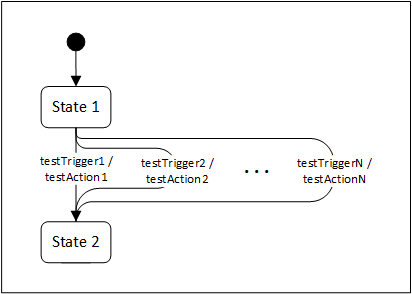
\includegraphics[width=80mm, keepaspectratio]{figures/validationStatechart.png}
	\caption{Schematic statechart of the proposed validation models}
	\label{fig:validationStatechart}
\end{figure}

During the testing of the individual language elements, one such statechart was implemented for each of the main constructs. To each of these statecharts belogs a Java test class, with one test case testing one of the transitions of the statechart against its expected behavior. An example of one such test case can be seen in Table \ref{tab:ValidationExample}.

It is important to note, that tests implemented this way are black-box tests -- i.e. they only test the functionality, not the implementation of the tested elements for two reasons. Firstly, they do not test the individual steps of the transformation workflow. Secondly, only the public interfaces of the generated Java classes are tested, which means, that we can only test event raisings directly (and the other elements only through events). On one hand, this is beneficial, as we are able to gain information on the (in)correctness of the individual language elements despite the number of tests remaining relatively small. On the other hand, whenever a tested functionality fails, there is no information provided about the cause of the problem, thus the correction of the code requires significantly higher effort.

The results of the validation of the individual language elements at the time of the writing this thesis are summarized in Table \ref{tab:ValidationTable}.

\begin{table}[H]
	\footnotesize
	\centering
	\begin{tabular}{ p{7cm} p{7cm} }
		\toprule
		Functionality to test & The corresponding test case \\
		\midrule
		\begin{lstlisting}
		//To test: in case of two branches of
		//an if statement are executable,
		//the earlier defined one is chosen
		
		transition from state1 to state2 
				when Input.ifG1elsifG2TrueLit / {		
			raise Output.pre;
			
			if (true) {
				raise Output.ifG1elsifG2_A;	
			} 
			elsif (true) {
				raise Output.ifG1elsifG2_B;
			}
			
			raise Output.ifG1elsifG2_C;
		}\end{lstlisting} & 
		\begin{lstlisting}
		@Test
		void testIfStatementStatechartIFG1elsifG2TrueLit() {
			// Arrange
			IfStatementStatechart sc =
					 new IfStatementStatechart();
			IfStatementStatechartInterface 
					scInterface = sc;
			
			// Act
			scInterface.reset();
			
			scInterface.getInput()
				.raiseIfG1elsifG2TrueLit();;
			scInterface.runCycle();
			
			// Assert
			Assertions.assertTrue(sc.getOutput()
				.isRaisedPre());
			Assertions.assertTrue(sc.getOutput()
				.isRaisedIfG1elsifG2_A());
			Assertions.assertFalse(sc.getOutput()
				.isRaisedIfG1elsifG2_B());
			Assertions.assertTrue(sc.getOutput()
				.isRaisedIfG1elsifG2_C());
		}\end{lstlisting} \\
		\bottomrule
	\end{tabular}
	\caption{Testing the execution of the correct branch of an if statement}
	\label{tab:ValidationExample}
\end{table}

%\newpage
%----------------------------------------------------------------------------
\section{Case study: RPN Calculator} \label{section_results_caseStudy}
%----------------------------------------------------------------------------
This section demonstrates the capabilities the action language. It presents a problem commonly solved in general-purpose imperative programming languages, offers a possible solution using statecharts of the Gamma Framework -- extended with the action language described in this thesis -- and evaluates the generated executable and verifiable code.
%----------------------------------------------------------------------------
\subsection{Introduction}
%----------------------------------------------------------------------------
The problem to solve is the parsing and evaluation of a mathematical expression that can contain integer numbers and basic arithmetical symbols (+, -, *, /). For the input to be valid for calculation, the expression must be a valid mathematical formula given with reverse polish (postfix) notation \cite{ParenthesesFreeNotation}. The calculator should be able to check the validity of the formula and signal an error in case it was invalid, or evaluate the formula, return the result and signal success if it was valid. 

It would also be worthwhile to design a tester component in addition to the calculator, which generates a valid input sequence and feeds it to the calculator on its input port. This would allow the users to observe the behavior of the calculator without having to produce the input themselves.
%----------------------------------------------------------------------------
\subsection{Designing the system}
%----------------------------------------------------------------------------
\textbf{The ports of the system:}
To implement the above described system, we require an interface, through which we can signal the tester to start feeding input to the calculator. We also wish to observe the result of the calculation, for which we provide an interface to the system. Our input should be sent through an interface provided by the tester, and the output should arrive on an interface provided to the calculator. The tester should be connected to the calculator through the input interface provided by the calculator and required by the tester. 

The input interface of the system (and also the tester), \textit{TesterInput}, only needs one type of event to \textit{start} the operation. The output interface of the system (also the calculator) can signal two different events: \textit{success} and \textit{error}. The interface of the calculator, \textit{CalcInput}, can take three different inputs: a single \textit{operator}, a single \textit{operand}, or the \textit{evaluate} command.

The components of the system and their connections are summarized on Figure \ref{fig:calculatorComponents}.

\begin{figure}[!ht]
	\centering
	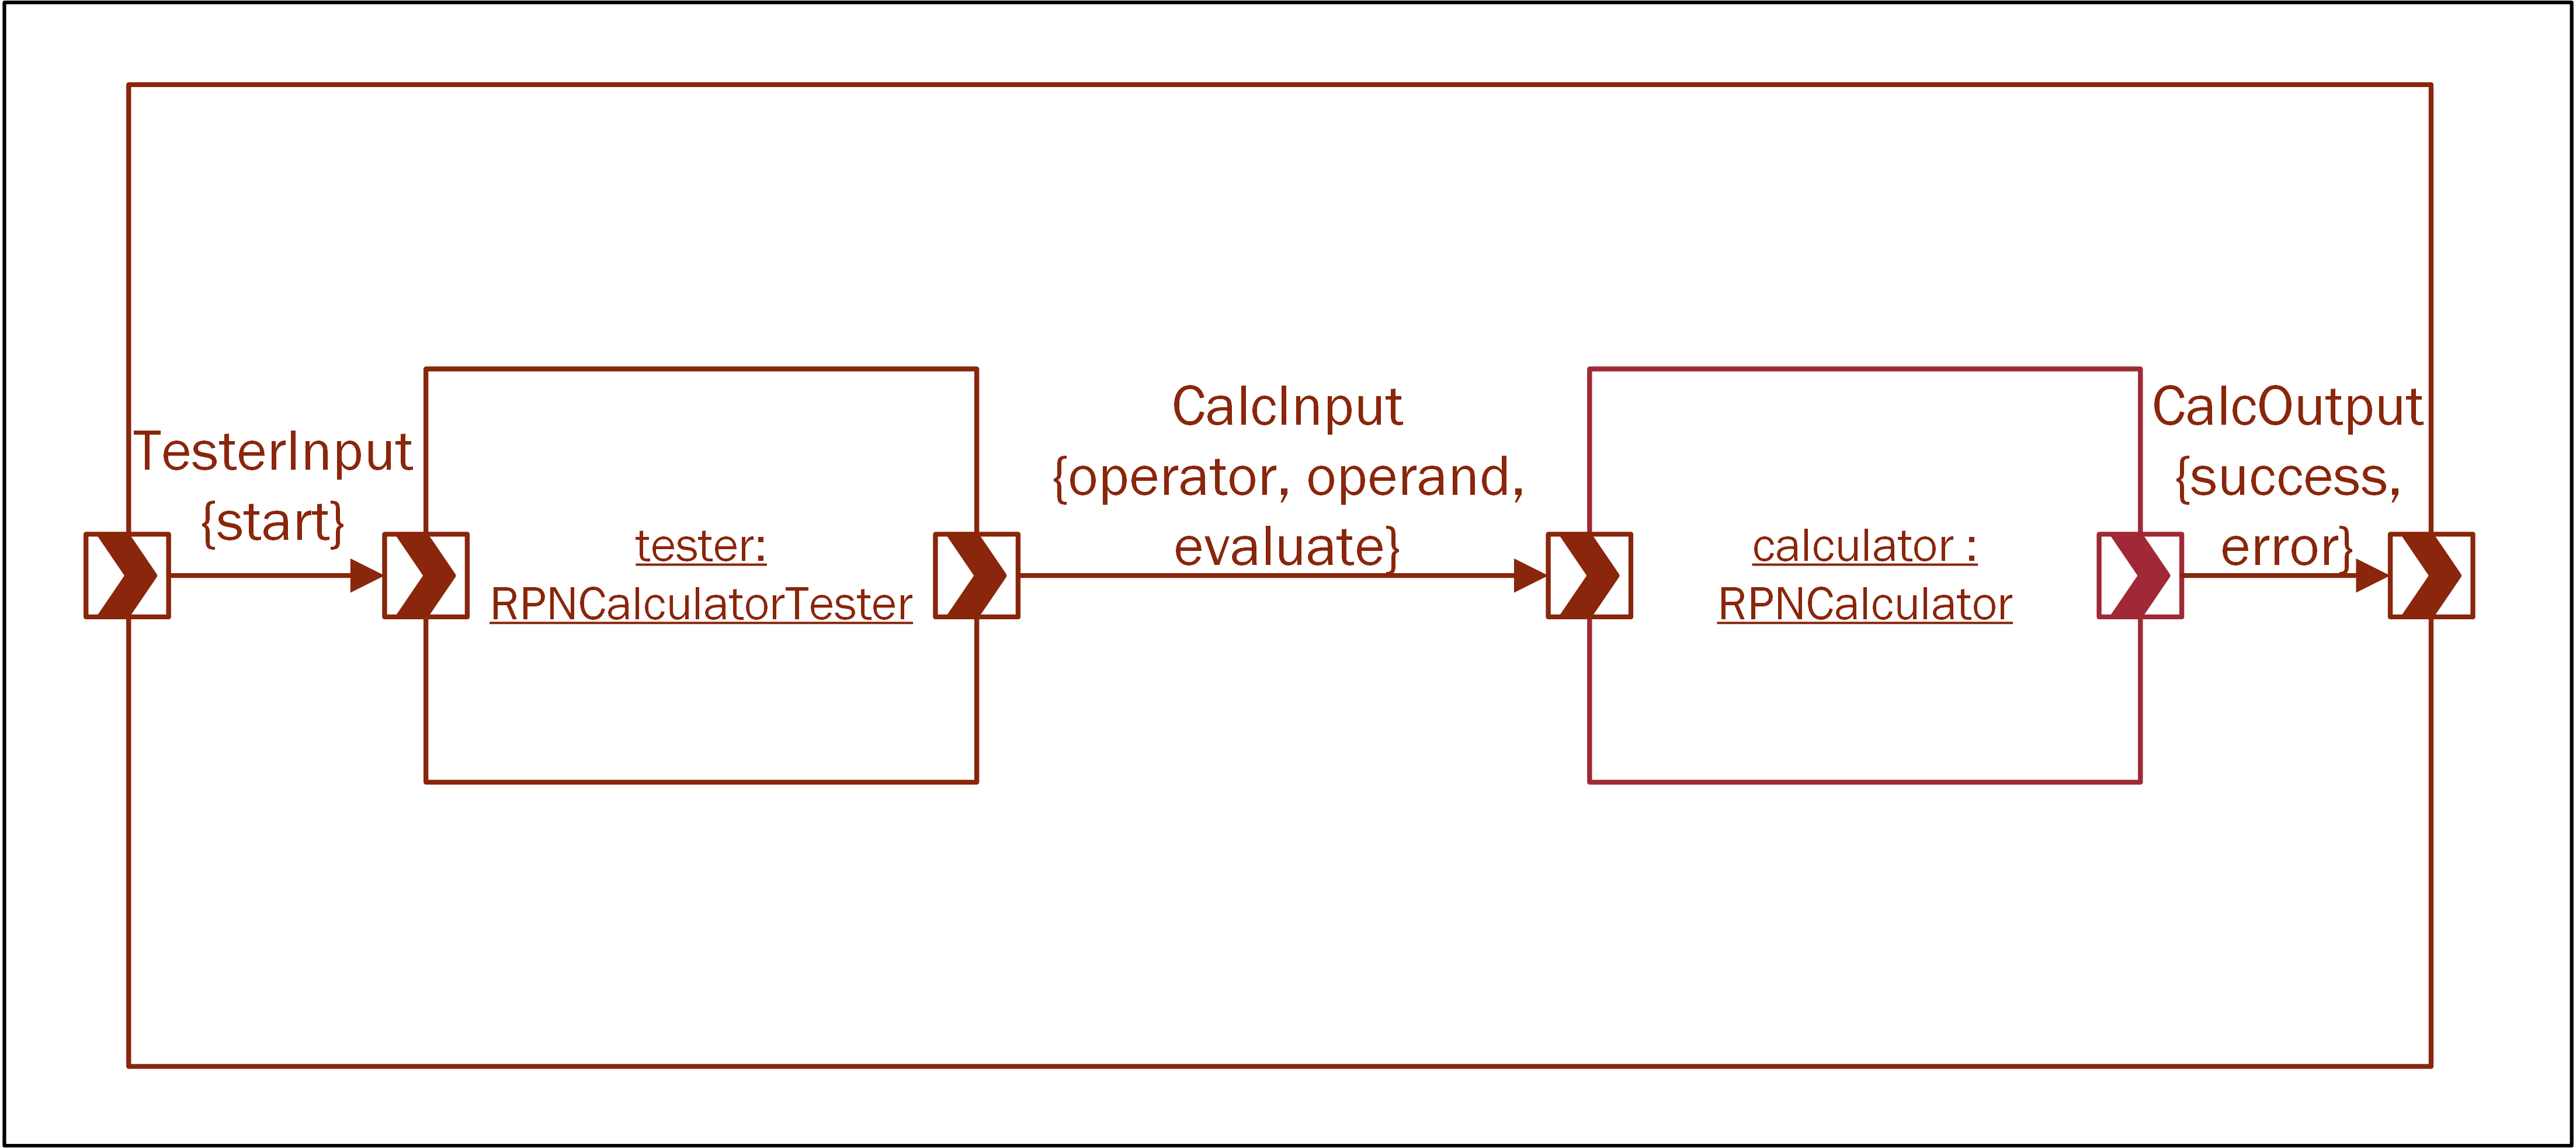
\includegraphics[width=150mm, keepaspectratio]{figures/calculatorComponents.png}
	\caption{Component diagram of the modeled system}
	\label{fig:calculatorComponents}
\end{figure}

\textbf{The states of the calculator:}

A formula is valid according to the rules of postfix notation, if it starts with two operands (or contains only one operand altogether), ends with an operator, and contains one less operators than operands -- as each possible operator takes two operands. As we are modeling the system using statecharts, the states of the system present a convenient way to verify the validity of the given expressions. The calculator should start in an initial state (\textit{'Init'}), which represents a state where the list of inputs is empty. As one number is considered a valid expression, there should be a state (\textit{'OneNumber'}) representing the validity of expressions consisting of only one operand. In this case, the logic of the evaluation is simple, as only that number needs to be returned. Apart from this special case, the expression should start with two numbers, but two operands without an operator are considered invalid (\textit{'Invalid'}). In the later phases, the system should return to this state, whenever the expression ends with an operand, as the expression should end with an operator. If the expression ends with an operator, the formula \textit{may} be considered valid (\textit{'MaybeValid'}), as the determination of the validity requires further computation.

\newpage
\textbf{The transitions of the calculator:}

In each possible state of the system, a transition should be defined for each of the possible inputs, as every input should result in some kind of behavior (even as simple as saving the input). In general, there are three kinds of different behaviors: when the formula is invalid and cannot become valid anymore, or when the evaluation of an invalid formula is required, the system should return to its initial state, clearing the previously saved data, and send an error on the output interface. When the formula may at one point in the future be considered valid, the input should be saved and the states should represent the current validity. When the formula is valid and an evaluation is required, the system should calculate and return the result and clear the stored input. The statechart representation of the calculator can be seen on Figure \ref{fig:calculatorStatechart}.

\begin{figure}[!h]
	\centering
	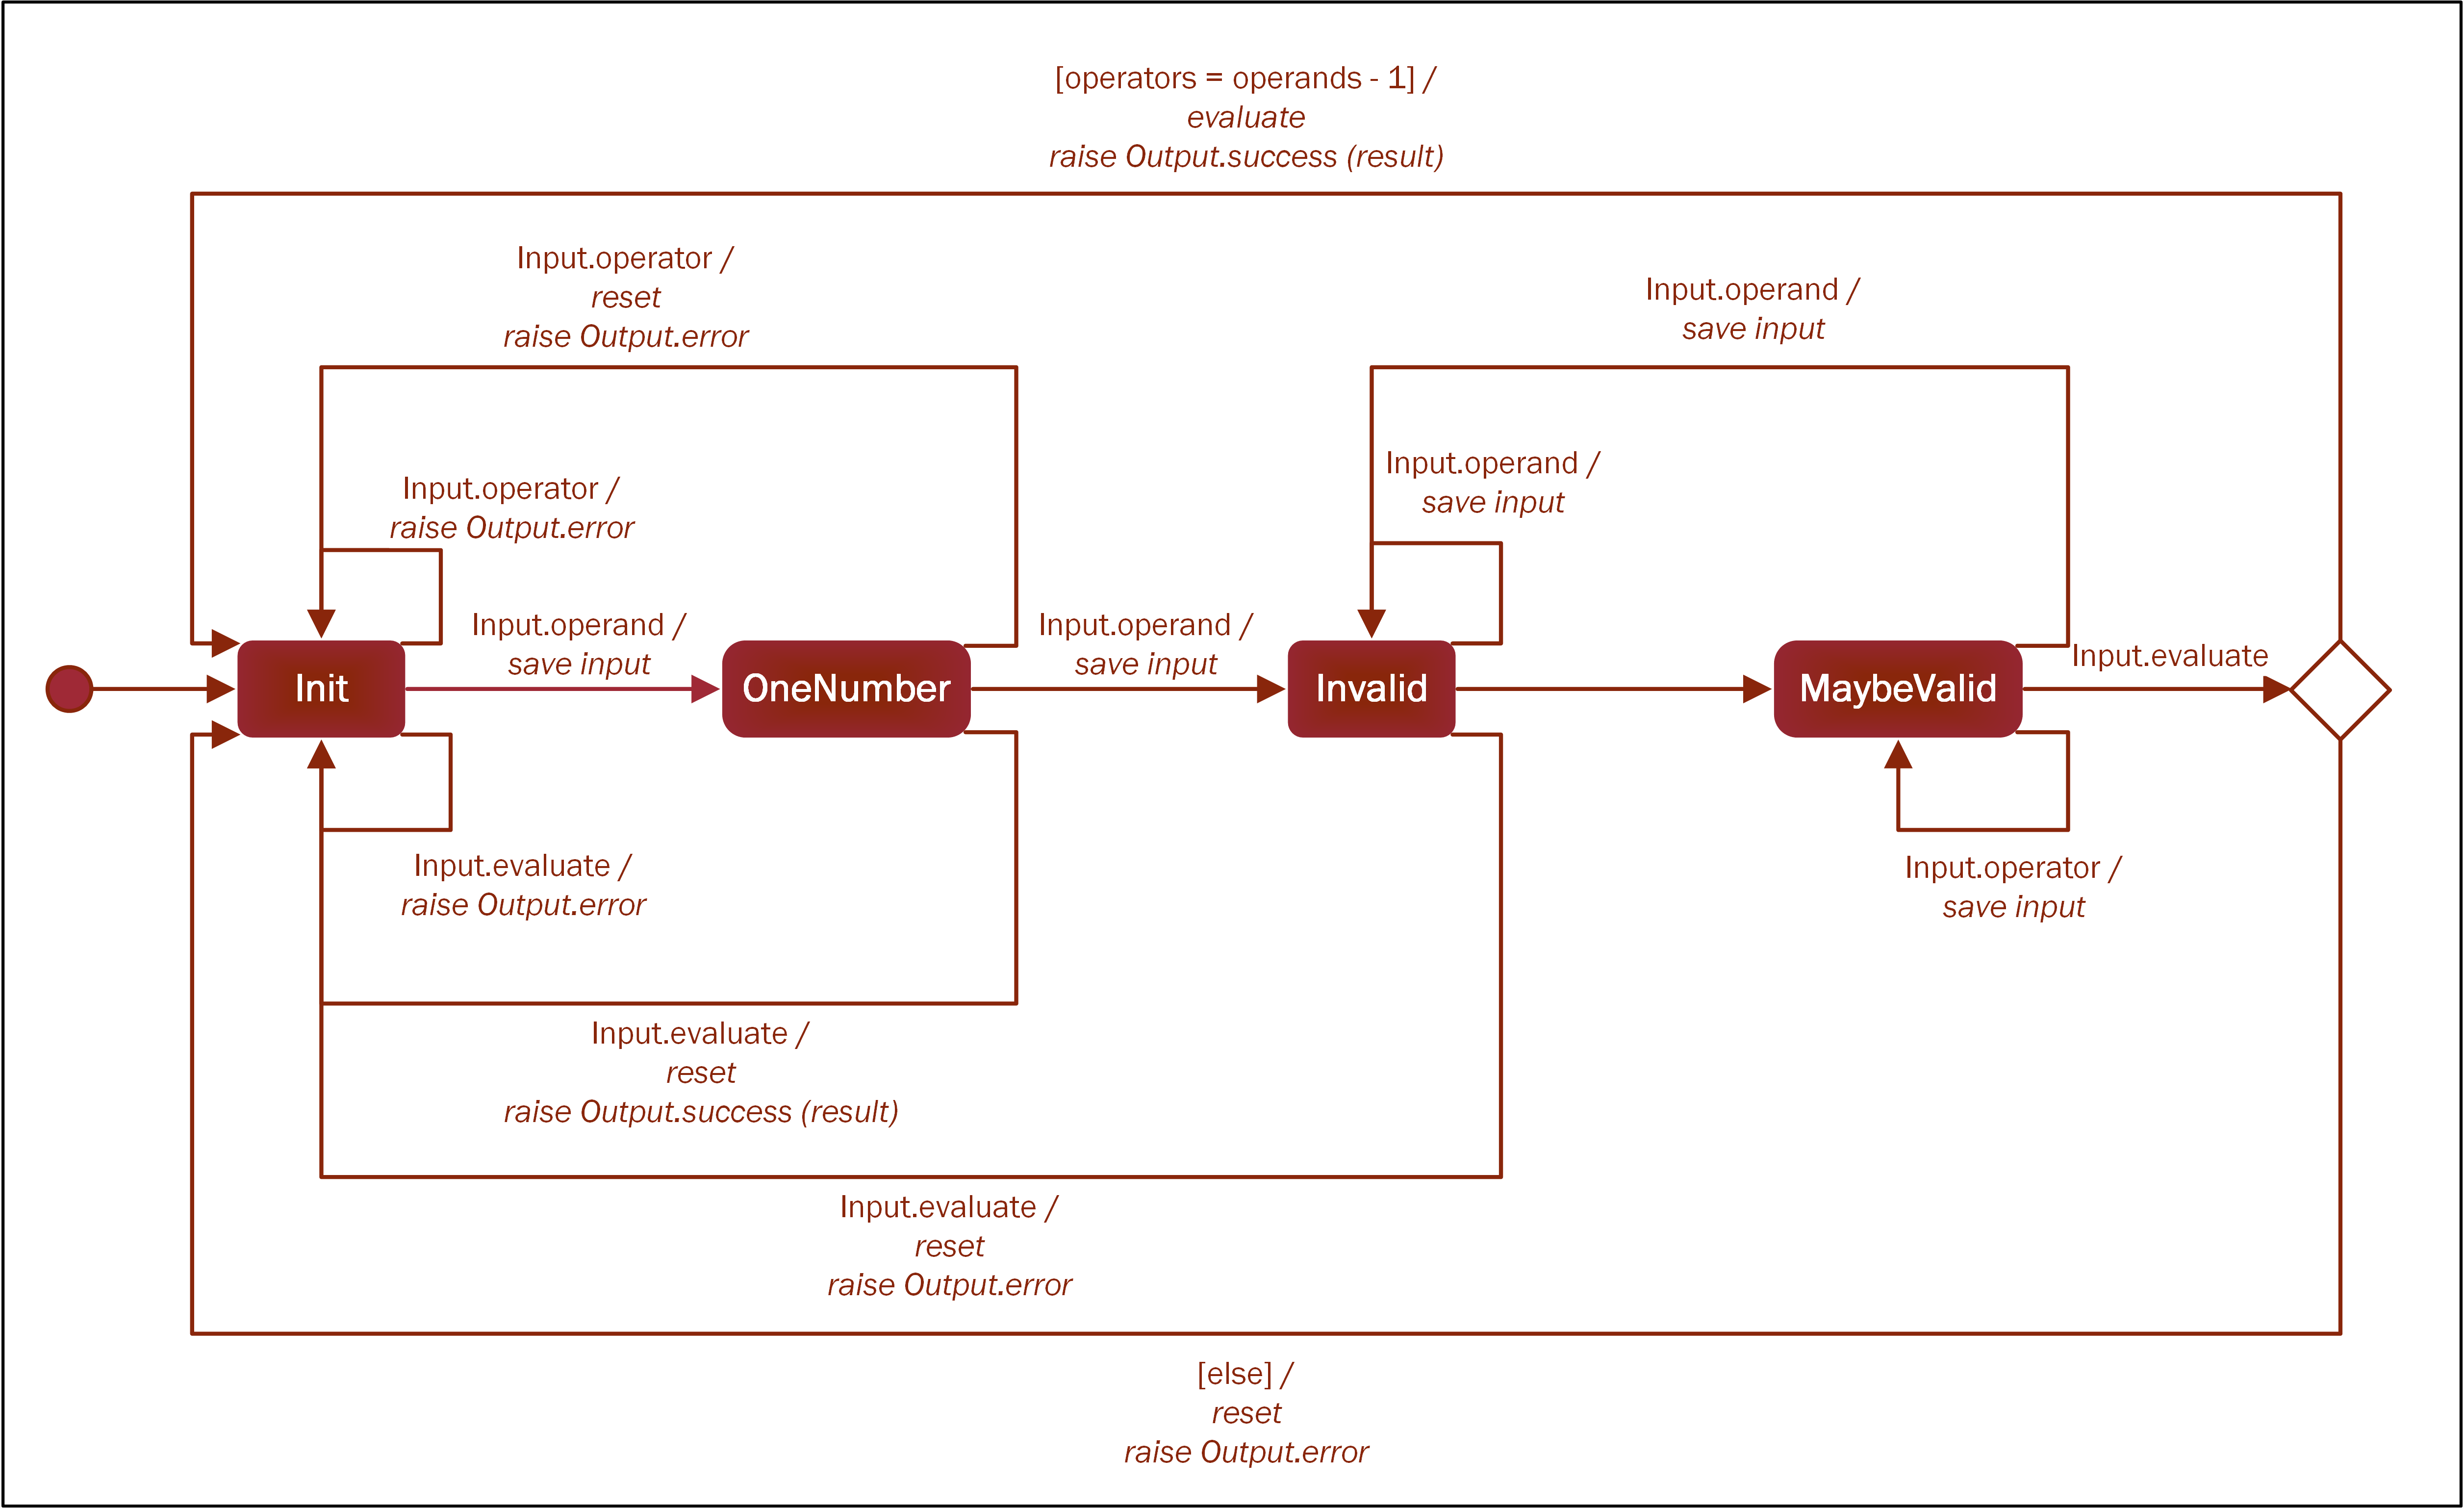
\includegraphics[width=150mm, keepaspectratio]{figures/calculatorStatechart.png}
	\caption{Statechart of the calculator}
	\label{fig:calculatorStatechart}
\end{figure}

\bigskip
\textbf{The tester:}

The structure and behavior of the tester is very simple, it only consists of two states, one possible input event, one timeout event and three possible output events. The statechart representation of the tester can be seen on Figure \ref{fig:testerStatechart}.

\begin{figure}[!h]
	\centering
	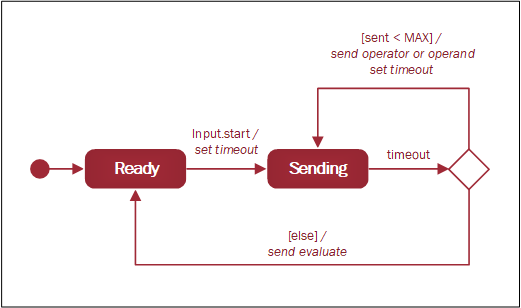
\includegraphics[width=90mm, keepaspectratio]{figures/testerStatechart.png}
	\caption{Statechart of the tester}
	\label{fig:testerStatechart}
\end{figure}

On the figures, the actions have been marked with \textit{italics}. 

%----------------------------------------------------------------------------
\subsection{The Gamma Model}
%----------------------------------------------------------------------------
The details of implementing the statecharts and their interfaces are omitted here, only those parts are included, which are directly needed to provide a context for the described actions. The rest of the system can be implemented according to Figures \ref{fig:calculatorComponents}, \ref{fig:calculatorStatechart} and \ref{fig:testerStatechart}. For the full implementation of the calculator module and its interfaces, see Listings \ref{lst:RPNCalculatorInterfacesSource} and \ref{lst:RPNCalculatorModelSource}.

\textbf{The applied data structures:} for the implementation we use the currently supported data structures, and also consider their current limitations. The inputs are stored in three separate arrays: one for the operators (\textit{operators}), one for the operands (\textit{operands}), and one for storing the sequence of operators and operands using boolean values (\textit{isOperator}). To simulate a stack-like functionality, we also declare three integer valued variables (\textit{numOperators, numOperands and numIsOperator}) and also keep in mind the maximum sizes of the arrays (2-2-4).   

\bigskip
\textbf{Transitions of the calculator component:}
As described in the previous sections, when considering the actions of the system, there are basically three different types of transitions: the ones \textit{saving the input}, the ones \textit{resetting the calculator and signaling error} and the one \textit{evaluating the provided expression and signaling success}. 

\textbf{Saving the input:} these transitions behave based on the input being an operator or an operand. Generally, they save the input into the corresponding array, at the place specified by the current state of the corresponding \textit{num} variable. They also add a boolean value to the \textit{isOperand} array at the place specified by the \textit{numIsOperand} variable. Then they increase each of the used \textit{num} variables to prepare it for the next input. The code describing this functionality can be seen in Listing \ref{lst:RPNSaveTransition}.

\bigskip
\begin{lstlisting} [language=tex,caption=Transition saving an input operand,label=lst:RPNSaveTransition]
	transition from OneNumber to Invalid when Input.operand / {
		operands[numOperands] := Input.operand::inOperand;
		isOperator[numIsOperator] := false;
		numOperands := numOperands + 1;
		numIsOperator := numIsOperator + 1;
	}
\end{lstlisting}

Considering the language elements, this transition contains various assignment statements, assigning different values to elements of arrays and simple variables.

\textbf{Resetting the calculator and signaling error:} these transitions set all the \textit{num} variables to 0 and raise the \textit{Output.error} event. By this, the (virtual) 'stack pointers' are returned to the base of the stack, thus making the contents unreachable (as long as the stack pointers are used in the right way). The code describing this functionality can be seen in Listing \ref{lst:RPNResetTransition}.

\bigskip
\begin{lstlisting} [language=tex,caption=Transition resetting the system,label=lst:RPNResetTransition]
	transition from OneNumber to Init when Input.operator / {
		raise Output.error;
		numOperators := 0;
		numOperands := 0;
		numIsOperator := 0;
	}
\end{lstlisting}

Considering the language elements, this transition contains one (simple) event raising, and three (simple) assignment statements.

\textbf{Evaluating the input:} this transition implements the modified version of the RPN left-to-right algorithm \cite{ParenthesesFreeNotation}. The pseudocode of the original algorithm can be found in Listing \ref{lst:RPNLeftToRight}, to which only modifications regarding the applied data structures were introduced -- i.e. the original algorithm stores the data in one array, in this example we use three arrays, as described above. In short, the algorithm requires a stack, on which the results of the individual operations are stored. It checks the input sequence iteratively, and if the element is an operand, it pushes it onto the stack. If the element is an operator, it takes two elements from the stack and calculates the result according to the operator. When the end of the input sequence is reached, the stack contains only one element, which is the result of the calculation. After the evaluation, the result of the calculation is sent along with the success signal. In the end, the calculator is reset. The code implementing this functionality can be seen on Listing \ref{lst:RPNEvalTransition}.

\bigskip
\begin{lstlisting} [language=tex,caption=Transition evaluating the input sequence,label=lst:RPNEvalTransition]
	transition from MaybeValid to Init when Input.evaluate [numOperators = numOperands - 1] / {
		var finalResult : integer; 
		
		//left-to-right algorithm variables
		var resultStack : array integer[2];
		
		var stackTop : integer := 0;
		var operatorsTop : integer := 0;
		var operandsTop : integer := 0;
		var isOperatorValue : boolean;
		
		//variables in the for loop
		var temp0 : Operator;
		var temp1 : integer;
		var temp2 : integer;
		var temp : integer;
		
		for (i : integer in [0 .. 4]){	//for the maximum possible input sequence
			if (i < (numOperators + numOperands)) {	//if there is an input at the given index
				isOperatorValue := isOperator[i];
				if (isOperatorValue) {	//if the input was an operator, evaluate
					//get the operator and the operands
					temp0 := operators[operatorsTop]; operatorsTop := operatorsTop + 1;
					temp1 := resultStack[stackTop]; stackTop := stackTop - 1;
					temp2 := resultStack[stackTop]; stackTop := stackTop - 1;
					
					//calculate
					if (temp0 = ::addition) {
						resultStack[stackTop] := temp1 + temp2; stackTop := stackTop - 1;
					}
					else if (temp0 = ::subtraction) {
						resultStack[stackTop] := temp1 - temp2; stackTop := stackTop - 1;
					}
					else if (temp0 = ::multiplication) {
						resultStack[stackTop] := temp1 * temp2; stackTop := stackTop - 1;
					}
					else if (temp0 = ::division) {
						resultStack[stackTop] := temp1 div temp2; stackTop := stackTop - 1;
					}	
				}
				else {	//if the input was an operand, push
					temp := operands[operandsTop]; operandsTop := operandsTop + 1;
					resultStack[stackTop] := temp; stackTop := stackTop + 1;
				}
			}
			else {	//no more input, can break
				break;
			}
		}
		
		//get the final result and send
		finalResult := resultStack[0];
		raise Output.success(finalResult);
		
		//reset the calculator
		numOperators := 0;
		numOperands := 0;
		numIsOperator := 0;
	}
\end{lstlisting}

This transition demonstrates the capabilities of multiple complex language elements. It declares local variables, iterates over a range of values, breaks the iteration when the continuation does not modify the final result anymore, and carries out operations based on the values of variables. 

It is easy to see, that this solution is unnecessarily complex, and further optimizations would be possible to improve not only the readability, but also the performance of the system. This is due to the currently supported language elements and model transformations of the Gamma Framework. Nevertheless, some of these -- currently only theoretical -- improvements are discussed in Subsection \ref{ss_res_rpn_improvement}.

\textbf{The tester component:} for the tester component, we are not going to analyze the individual transitions, variables or data structures of the component, as there is no complex algorithm to implement when sending a \textit{random} input sequence. Instead, we are going to analyze implementation of the individual actions using the introduced action language.

The send operator and send operand actions can be implemented using choice or select statements: we want the operators and operands to be randomly selected from the possible values, and these constructs offer exactly that through non-deterministic choice. A possible implentation of these actions can be seen on Listings \ref{lst:TesterSendOperator} and \ref{lst:TesterSendOperand}.

\bigskip
\begin{lstlisting} [language=tex,caption=Sending a random operator to the calculator,label=lst:TesterSendOperator]
	{
		. . .
		choice {
			branch[true] raise Output.operator(::addition);
			branch[true] raise Output.operator(::subtraction);
			branch[true] raise Output.operator(::multiplication);
			branch[true] raise Output.operator(::division);
		}
		. . .
	}
\end{lstlisting}
\bigskip
\begin{lstlisting} [language=tex,caption=Sending a random operand to the calculator,label=lst:TesterSendOperand]
	{
		//var toSend : integer;
		. . .
		toSend := [0 .. 100].select; //selecting a number between 0 and 100
		raise Output.operand(toSend);
		. . .
	}
\end{lstlisting}

%----------------------------------------------------------------------------
\subsection{Evaluation of the Results}
%----------------------------------------------------------------------------
The calculator component of the designed system was implemented using the Gamma Framework. The AST was correctly constructed from the textual description of the statechart, and no elements were marked incorrect by the validation rules. However, the model transformations (to low-level statechart, then to xSTS, then to Java) yielded unexpected results.

To provide a basis of comparison, the execution of the transformation workflow for the validation models discussed in Section \ref{section_results_validation} on a given setup only lasted a few seconds and resulted in .java files under 1MB.

In case of the RPN Calculator, the execution of the model transformations on the same setup, with the modeled system only able to add two numbers lasted around two minutes and resulted in a ~16MB .java file. For a calculator able to add or subtract two numbers, the transformations lasted around twenty minutes and resulted in a ~76MB .java file. The .java files contained no errors apart from the size of an individual method exceeding the maximum ~64kB size or the OutOfMemoryExceptions when trying to compile the given file.

\textbf{The problem:} during the model transformations, many brute-force solutions are applied. These solutions include, but are not limited to local variables not being differentiated from global variables, array access expressions being implemented using additional variable declarations and if-statements consisting of several branches, and guards of if, choice and switch statements being extracted into separate variables and assignments, to be able to support access expressions. These actions result in the state space explosion of the system. This leads to many complex transitions, which are then merged into one xSTS transition, which is in turn transformed into one Java method that is impossible to compile and execute -- even though the transformation and the resulting operation of the individual elements may be correct.

%----------------------------------------------------------------------------
\subsection{Further Improvements of the Calculator} \label{ss_res_rpn_improvement}
%----------------------------------------------------------------------------
If we assume that all the language elements are integrated into the Gamma Framework as described in Chapter \ref{chapter_theoreticalResults}, we can improve the calculator in several ways: 
\begin{itemize}
	\item The input can be stored in one array of records, eliminating the need for the modification of the left-to-right algorithm, thus making the code more efficient and readable.
	\item A stack type can be implemented using records containing an array and an integer, the latter containing the top of the stack.
	\item Variables can be declared inside a for-loop, making the code easier to understand.
	\item Variables can be assigned complex expressions (e.g. array access) in their initializer expressions, reducing the number of statements needed.
	\item The input evaluation logic can be extracted into a procedure, making the code more readable.
	\item The operation evaluation logic can be extracted into a procedure, making the code more readable.
\end{itemize}

These modifications are currently not possible, as either the language, or the model transformations of the framework do not support them. However, the model could be further refined using the currently supported elements too: for instance, input buffer overflow is not handled by the given code.